\begin{tikzpicture}[scale=.85]


  \def\labels{ c, b, a, p, o, n, m, l, k, j, i, h, g, f, e, d}
  
  \def\reward{88.3,86.3,88.1,74.5,77.6,78.6,85.0,73.0,73.3,83.1,64.0,54.9,84.0,75.0,62.0,85.2}
  \def\dbSize{32,20,76,488,118,20,50,400,6,120,25,352,347,480,42,20}
  \def\dbClass{1,1,2,3,2,1,2,3,1,2,1,3,3,3,1,1}		
  \def\cZoom{3} 
  \def\percentageLabelAngle{90}
  \def\nbeams{16}
  \pgfmathsetmacro\beamAngle{(360/\nbeams)}
  \pgfmathsetmacro\halfAngle{(180/\nbeams)}
  % \def\globalRotation{10}
  \pgfmathsetmacro\globalRotation{\halfAngle}

  % draw manual AOV results
  \filldraw[aov!15!white,even odd rule] (0,0) circle [radius={\cZoom*.852}] (0,0) circle [radius={\cZoom*.8}];
  \draw[thin,color=aov!50!white,dashed] (0,0) circle [radius={\cZoom*.852}] (0,0) circle [radius={\cZoom*.8}];

  % \foreach \x in {.125,.25, ...,1} { \draw[thin]  (0,0) circle [radius={2*\x}]; }
  % draw the radiants with the reference label
  \foreach \n  [count=\ni] in \labels
  {
    \pgfmathsetmacro\cAngle{{(\ni*(360/\nbeams))+\globalRotation}}
    \draw [thin] (0,0) -- (\cAngle:{\cZoom*1}) ;
    \draw	(\cAngle:{\cZoom*1.1})  node[fill=white, inner sep=0pt] {{\tiny \textbf  \n}}; %referencies
  }

  % draw the % rings 
  \foreach \x in {12.5,25, ...,100} 
  \draw [thin,color=gray!50] (0,0) circle [radius={\cZoom*\x/100}];

  \foreach \x in {50,75,100}
  { 
    \draw [thin,color=black!50] (0,0) circle [radius={\cZoom/100*\x}];
    \foreach \a in {0, 180} \draw ({\percentageLabelAngle+\a}:{\cZoom*0.01*\x}) node  [inner sep=0pt,outer sep=0pt,fill=white,font=\fontsize{5}{5}\selectfont]{$\x$};
  }
  
  %% draw our results ring
  \draw [thick,color=black] (0,0) circle [radius={\cZoom*.63}];
  \foreach \a in {0, 180} \draw ({\percentageLabelAngle+\a}:{\cZoom*0.63}) node  [inner sep=0pt,outer sep=0pt,fill=white,font=\fontsize{5}{5}\selectfont]{$62.3$};


  % draw the path of the percentages
  \def\aux{{\reward}}
  \pgfmathsetmacro\origin{\aux[\nbeams-1]} 
  \draw [aov, thick] (\globalRotation:{\cZoom*\origin/100}) \foreach \n  [count=\ni] in \reward { -- ({(\ni*(360/\nbeams))+\globalRotation}:{\cZoom*\n/100}) } ;

  % label all the percentags
  \foreach \n [count=\ni] in \dbSize 
  {
    \pgfmathsetmacro\cAngle{{(\ni*(360/\nbeams))+\globalRotation}}
    \pgfmathsetmacro\nreward{\aux[\ni-1]}
%    \draw (\cAngle:{\cZoom*1.4}) node[align=center] {{\color{aov}\nreward $\%$} \\ {\color{db}\n} };
  } ;

  % draw the database rose
  \def\dbScale{\09}
  \foreach \n [count=\ni] in \dbClass
  \filldraw[fill=db!20!white, draw=db!50!black]
  (0,0) -- ({\ni*(360/\nbeams)-\halfAngle+\globalRotation}:{\cZoom*\n/9}) arc ({\ni*(360/\nbeams)-\halfAngle+\globalRotation}:{\ni*(360/\nbeams)+\halfAngle+\globalRotation}:{\cZoom*\n/9}) -- cycle;
  \foreach \x in {1,2,3}
  \draw [thin,color=db!50!black,dashed] (0,0) circle [radius={\cZoom*\x/9}];

  %% draw the legend
  \node [anchor=north west,yshift=-6pt] at (-45:\cZoom*1.1){
    \begin{tikzpicture}[font=\tiny]
      \begin{customlegend}[ 
        legend style={ draw=none},
        legend entries={AOV, Result}
        ]
        \addlegendimage{db,draw=aov,thick,sharp plot}
        \addlegendimage{db,draw=black,thick,sharp plot}
      \end{customlegend}
    \end{tikzpicture}};

  \node [anchor=north east, xshift=-5pt] at (-130:\cZoom*1.1){
    \begin{tikzpicture}[font=\tiny]
      \begin{customlegend}[ 
        legend style={ draw=none},
        legend entries={Dataset, Experts\cite{gerard2013}}
        ]
        \addlegendimage{db,fill=db!20!white, draw=db!60!gray, ybar, ybar legend}
        \addlegendimage{db,fill=aov!15!white,draw=aov,dashed,area legend}
      \end{customlegend}
    \end{tikzpicture}};

  %% draw the domain of each class 
  %\def\puta{	3/0/{\tikz{\node[nodeBase,acmStyle]{};}ACM},
  \def\puta{	3/0/{ACM},
    3/3/{ACM+Other},
    3/6/{Other}}
  \def\putaa{  	2/9/{Other+ML},
    3/11/{ML},
    2/14/{ML+ACM}}

  \foreach \numElm/\contadorQueNoSeCalcular/\name [count=\ni] in \puta
  {

    \pgfmathsetmacro\initialAngle{(\contadorQueNoSeCalcular*\beamAngle)+\halfAngle+\globalRotation}
    \pgfmathsetmacro\finalAngle  {((\numElm+\contadorQueNoSeCalcular)*\beamAngle)+\halfAngle+\globalRotation}
    \pgfmathsetmacro\l  {\cZoom*1.1+.3pt}
    \draw (\initialAngle:{\cZoom*1.1}) -- (\initialAngle:{\cZoom*1.1});
    \draw [ |<->|,>=latex] (\initialAngle:\l) arc (\initialAngle:\finalAngle:\l) ;
    \pgfmathsetmacro\r  {\cZoom*1.1+.45pt}
    {\draw [decoration={text along path,  text={\name},text align={center}},decorate] (\finalAngle:\r) arc (\finalAngle:\initialAngle:\r);}
  }
  
  \node[nodeBase,acmStyle] at (63:\cZoom*1.28) {};
  \node[nodeBase,mlStyle] at (-61:\cZoom*1.28) {};
  \node[nodeBase,otherStyle] at (-161.5:\cZoom*1.28) {};

  \foreach \numElm/\contadorQueNoSeCalcular/\name [count=\ni] in \putaa
  {

    \pgfmathsetmacro\initialAngle{(\contadorQueNoSeCalcular*\beamAngle)+\halfAngle+\globalRotation}
    \pgfmathsetmacro\finalAngle  {((\numElm+\contadorQueNoSeCalcular)*\beamAngle)+\halfAngle+\globalRotation}
    \pgfmathsetmacro\l  {\cZoom*1.1+.3pt}
    \draw (\initialAngle:{\cZoom*1.1}) -- (\initialAngle:{\cZoom*1.1});
    \draw [ |<->|,>=latex] (\initialAngle:\l) arc (\initialAngle:\finalAngle:\l) ;    									 
    \pgfmathsetmacro\r  {\cZoom*1.1+.61pt}
    {\draw [decoration={text along path, text={\name},text align={center}},decorate] (\initialAngle:\r) arc (\initialAngle:\finalAngle:\r);}    			 
  }
  
  \node[] at (5.8,3) 
  {\tiny \newcommand{\myCoord}[1]{
  \tikz[remember picture]{\coordinate[remember picture] (#1) at (0,0);
    %\fill[red] (#1) circle[radius=1pt];
  }
}


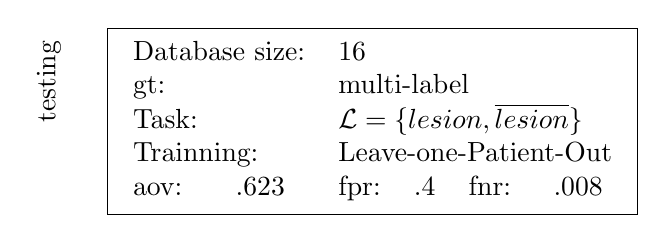
\begin{tikzpicture}[remember picture]
  \tikzstyle{noMargin} = [inner sep=0mm, outer sep=0mm]
  %\node[draw, noMargin, remember picture, anchor=north west,
  %minimum width = 3cm,
  %label={[label distance=-0.8cm,text depth=15pt,rotate=90]left:description}
  %](methodTech){
  %  \qquad
  %  \begin{tabular}{lll}
  %    \multicolumn{3}{l}{technology used for:}\\ 
  %    \multicolumn{2}{l}{\qquad detection}& \myCoord{mlInit}\\
  %    \multicolumn{2}{l}{\qquad segmentation}\\
  %    \multicolumn{2}{l}{\qquad post-processing}&\myCoord{mlFin}\\
  %    $\mathcal{S}$: & \multicolumn{2}{l}{Quick-Shift super-pixels}\\
  %    $\arg \min (U(\cdot))$:&\multicolumn{2}{l}{\acl{gc}}\\
  %    $D(\cdot)$:&\multicolumn{2}{l}{\tikz[noMargin, baseline=(img.north)]{\node[noMargin](img){\includegraphics[width=1cm]{vcues}};}}\\
  %    &\multicolumn{2}{l}{\acs{rbf}-\acs{svm}}\\
  %    $V(\cdot,\cdot)$:&\multicolumn{2}{l}{Homogenity}\\
  %  \end{tabular}
  %};
  %\node[yshift=2pt,remember picture, overlay, nodeBase, mlStyle, fit= (mlInit) (mlFin)]{};
\node[draw, %below= 2pt of methodTech,
minimum width = 3.9cm,
  label={[label distance=-0.5cm,text depth=15pt,anchor=south, rotate=90]left:testing}
  ](testingNode){
    \begin{tabular}{lclclc}
      \multicolumn{2}{l}{Database size:} & \multicolumn{4}{l}{$16$} \\
      \multicolumn{2}{l}{\ac{gt}:}       & \multicolumn{4}{l}{multi-label} \\
      \multicolumn{2}{l}{Task:}          & \multicolumn{4}{l}{$\mathcal{L} = \{\text{lesion}, \overline{\text{lesion}}\}$} \\
      \multicolumn{2}{l}{Trainning:}     & \multicolumn{4}{l}{Leave-one-Patient-Out}\\
      \ac{aov}:      & .623                                                                               & \acs{fpr}: & .4 & \acs{fnr}: & .008
    \end{tabular}
    };
%  \node[
%        draw=red,
%        minimum width=\textwidth,
%        fit=(current bounding box.north west) (current bounding box.south east),
%      ]at (current bounding box.center){};
\end{tikzpicture}

};
\end{tikzpicture}
